
\section{CAN Communication Protocol}

The controller area network (CAN) is a highly integrated system that connects intelligent devices for  real-time control applications by utilizing serial bus and communications protocol. Control Area Network use a vehicle bus standard that allows communication such as, transferring messages, data or informations between micro-controllers and other devices. CAN is able to operate at data speeds of up to 1 megabits per second (1Mbps) over a possible line length of up to several kilometres, and has outstanding error detection and confinement capabilities. Control Area Network which is also well-known as CAN Communication was introduced by Robert Bosch GmbH in 1983. CAN is purposely created to make automobile industry system more reliable and efficient but it is also widely used in industrial automation and other fields. 
\subsection{The CAN Standard }

The International Organization for Standardization (ISO) designed the CAN serial communications bus for the automotive industry to replace the complex wiring harness with a two-wire bus. According to the standard, high immunity to electrical interference is necessary, as well as the capacity to self-diagnose and correct data errors. CAN is widely utilized in a variety of industries, including building automation, medical, and manufacturing, because to these qualities.


\begin{figure}[h]
    \centering
    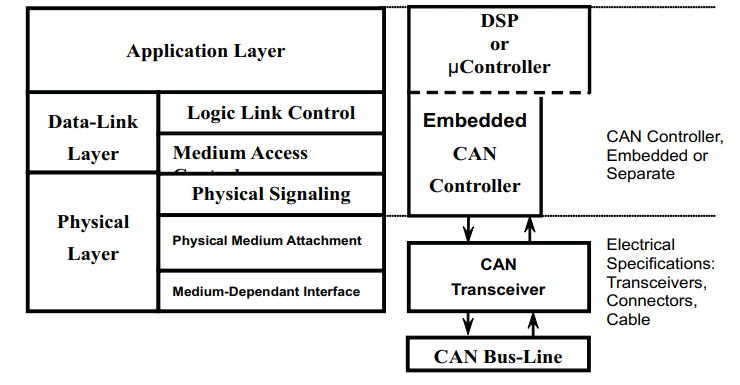
\includegraphics[width=0.5\textwidth]{standard}
    \caption{The Layered ISO 11898 Standard Architecture \cite{b5}}
    \label{fig:standard}
\end{figure}

The CAN communications protocol, ISO-11898: 2003, specifies how data is transmitted between devices on a network and follows the Open Systems Interconnection (OSI) paradigm, which is divided into layers. The physical layer of the model defines the actual communication between devices connected by the physical medium. as shown Figure \ref{fig:standard}

\subsection{Standard CAN }

The CAN communication protocol is a carrier-sense, multiple-access protocol (CSMA/CD+AMP) that includes collision detection and message priority arbitration. Each node on a bus must wait for a certain duration of idleness before attempting to send a message, according to CSMA. CD+AMP denotes that collisions are resolved using bit-wise arbitration, with each message's priority preprogrammed in the identification field. Bus access is always granted to the identification with the highest priority. That example, because the last logic high in the identification has the highest priority, it continues to transmit. An arbitrating node knows if it placed the logic-high bit on the bus because every node on the bus participates in writing every bit "as it is written."

\subsection{A CAN Message }
\subsubsection{Arbitration}

The opposing logic state between the bus and the driver input and receiver output is a basic CAN property, as shown in Figure 4. A logic high is normally linked with a one, and a logic low with a zero, however this is not the case on a CAN bus. This is why the driver input and receiver output pins of TI CAN transceivers are internally passively pushed high, such that the device defaults to a recessive bus state on all input and output pins in the absence of any input.

Bus access is based on events and occurs at random. If two nodes try to occupy the bus at the same time, nondestructive bit-wise arbitration is used to provide access. Nondestructive means that the node that wins arbitration keeps sending the message without it being deleted or corrupted by another node.

A feature of CAN that makes it particularly appealing for application in a real-time control environment is the allocation of priority to messages in the identification. The higher the priority, the smaller the binary message identifying number. Because it keeps the bus dominant the longest, a message with an identification made entirely of zeros is the highest priority message on a network. As a result, if two nodes start transmitting at the same time, the node that sends a zero (dominant) as the last identifying bit while the others send a one (recessive) holds control of the CAN bus and continues to complete its message. On a CAN bus, a dominant bit always overwrites a recessive bit.

\subsubsection{Message Types}
There are four different message types (or frames) that can be transmitted on a CAN system as below:

\begin{itemize}
\item The Data Frame
\item The Remote Frame
\item The Error Frame
\item The Overload Frame
\end{itemize}

\subsubsection{A Valid Frame}

When the last bit of a message's terminating EOF field is received in the error-free recessive state, the message is considered error-free. The transmitter repeats a broadcast if a dominating bit in the EOF field is present.

\subsubsection{Error Checking and Fault Confinement}

The abundance of error-checking mechanisms in CAN contributes to its robustness. The CAN protocol has five error-checking methods: three at the message level and two at the bit level. If a message fails to pass any of these error detection mechanisms, it is not accepted, and the receiving node generates an error frame. This compels the transmitting node to relay the message several times until it is appropriately received. If a malfunctioning node hangs up a bus by repeatedly repeating an error, its controller disables its transmit capacity if an error limit is reached.


1) Message Level


A form check is performed at the message level. This check examines the message for fields that must always be recessive bits. An error is generated if a dominating bit is discovered. The SOF, EOF, ACK delimiter, and CRC delimiter bits are all examined.

2) Bit Level


Each bit transferred is monitored at the bit level by the message's transmitter. An error is caused if a data bit (not an arbitration bit) is written onto the bus and its opposite is read. The message identity field, which is used for arbitration, and the acknowledge slot, which requires a recessive bit to be replaced by a dominant bit, are the only exceptions.

\subsection{The CAN Bus}

The CAN standard establishes a communication network that connects all bus nodes and allows them to communicate with one another. A central control node may or may not exist, and nodes may be added at any moment, even while the network is operational (hot-plugging)

\begin{figure}[h]
    \centering
    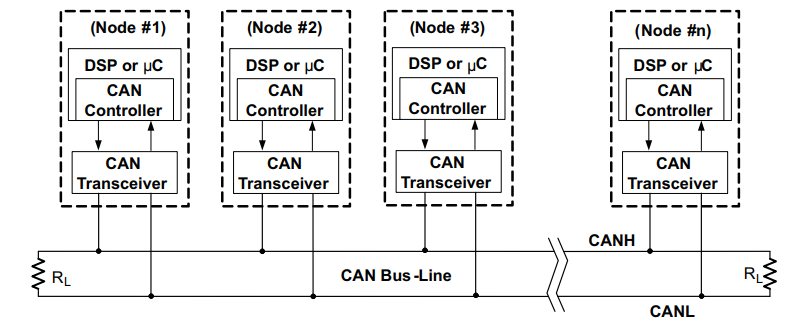
\includegraphics[width=0.5\textwidth]{CANbus}
    \caption{ Details of a CAN Bus \cite{b5}}
    \label{fig:CANbus}
\end{figure}



\subsubsection{CAN Transceiver Features}



1) 3.3V Supply Voltage

2) ESD Protection

3)Common- Mode Voltage Operating Range

4) Common-Mode Noise Rejection

5) Controlled Driver Output Transistion Times

6) Low-Current Bus Monitor, Standby and Sleep Modes

7) Low-Current Bus Monitor, Standby and Sleep Modes

8) Thermal Shutdown Protection

9)  Bus Input Impedance

10)  Glitch-Free Power Up and Power Down

11)  Unpowered Node Protection

12) Reference Voltage

13) V-Split

14) Loopback

15) Autobaud Loopback





 